\section{mbeddr Debugger Framework}
\label{mbeddrDebugger}
\label{mbeddrDebuggerFramework}

mbeddr comes with a debugger, which allows users to debug their mbeddr code 
on the abstraction levels of the used languages. For that, each language
contributes a debugger extension, which is build with a framework also provided
by mbeddr~\cite{DBLP:conf/adaEurope/AdaEuropeDeb}.
% will be fixed by aoun ! :-)
Debugging support is implemented specificly for the language by
lifting the call stack/program state from the base-level to the
extension-level (see \fig{infoFlow}) and stepping/breakpoints
vice versa.

\begin{figure}[h]
  \vspace{-2mm}
  \centering
    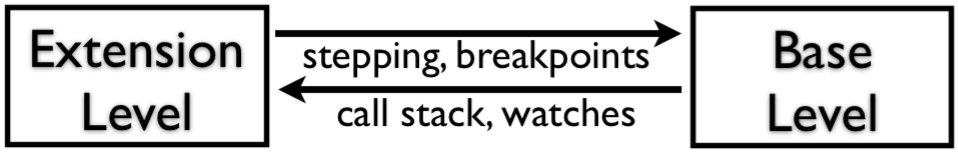
\includegraphics[width=5.5cm]{./figures/two-levels.png} 
    \vspace{-2mm}
    \caption{Flow of debug information between base and
    extension level~\cite{DBLP:conf/adaEurope/AdaEuropeDeb}}
  \label{infoFlow}
  \vspace{-2mm}
\end{figure}



The debugger framework can be separated into two different parts: First, a
\ac{DSL} and a set of interfaces (shown in \fig{specabs}) for specifying the
debugging semantics of language constructs. 
Second, a runtime for executing those specifications and
this way performing the mapping described in the~\fig{infoFlow}. 

You can find further information about the architecture and how it is
implemented with \ac{MPS} in \cite{DBLP:conf/adaEurope/AdaEuropeDeb}. In this
section we only discuss the specification part, which is essential for
understanding how to build a debugger extensions for our language example.

\noindent \textbf{Breakpoints} \ic{Breakable}s are concepts on which
we can set breakpoints (\eg \ic{Statement}s).

\noindent \textbf{Watchables} \ic{WatchProvider}s are
translated to low-level watchables (\eg \ic{GlobalVariableDeclaration}) or
represent watchables on the extension-level.
They are declared inside \ic{WatchProviderScope}s (\eg
\ic{StatementList}), which define their scope.

\noindent \textbf{Stepping} \ic{Steppable}s  
define where program execution must suspend
next, after the user \emph{steps over} 
an instance of \ic{Steppable} (\eg \ic{Statement}). If a
\ic{Steppable} contains a \ic{StepIntoable} (\eg \ic{FunctionCall}), 
then the \ic{Steppable} also supports \emph{step into}. \ic{StepIntoable}s are
concepts that branch execution into a \ic{SteppableComposite} (\eg \ic{Function}).
All stepping is implemented by setting low-level breakpoints and then resuming
execution until one of these breakpoints is hit (approach is based
on~\cite{Wu06grammar}).
Stepping-related concepts use \ic{DebugStrategies},
which implement a particular stepping behavior.

\noindent \textbf{Call Stack} \ic{StackFrameContributor}s are
concepts that have callable semantics on the extension-level or are
translated to low-level callables. While the latter do not
contribute any \ic{StackFrame}s to the high level call stack, the former
contribute at least one \ic{StackFrame}.

\begin{figure}[h]
  \vspace{-2mm}
  \centering
    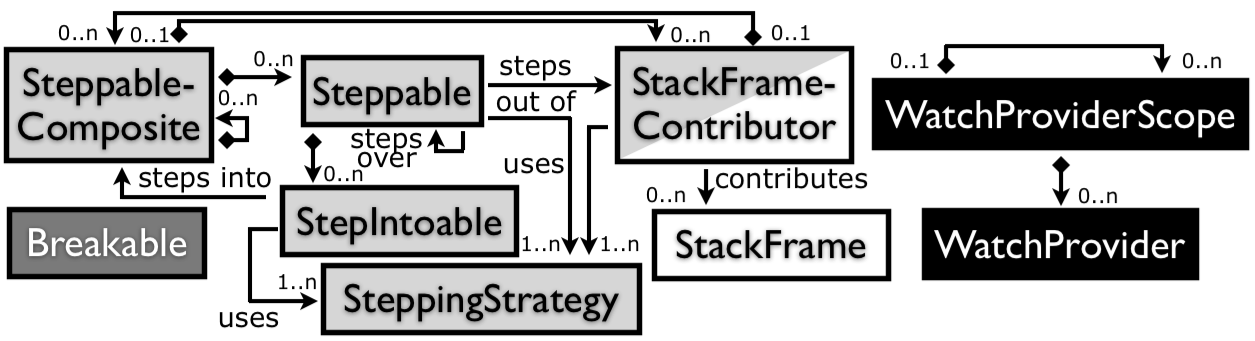
\includegraphics[width=9cm]{./figures/debugger-concepts.png} 
    \vspace{-2mm}
    \caption{Meta-model used for specying the debugging semantics of language
    constructs~\cite{DBLP:conf/adaEurope/AdaEuropeDeb}. Colors indicate the
    different aspects.} 
  \label{specabs}
  \vspace{-2mm}
\end{figure}

\section{Debugger Extension for Unit Testing}

We describe in this section the implementation of a minimal debugger
for our unit test lanuage. The debugger framework comes with a \ac{DSL}
for specifying the debugging behavior. We will use this \ac{DSL} and the
abstractions shown in \fig{specabs} for building the debugging support.

\parhead{Breakpoints}  We want to be able to set breakpoints on instances of
\ic{AssertStatement}. For being able to, we only need to implement the marker
interface \ic{IBreakable}. Since this concept
is derived from \ic{Statement} which already implements this
interface, we can already set breakpoints on instances of \ic{AssertStatement}.

\parhead{Call Stack} For lifting the call stack we need to specify, which
concepts have callable semantics or are generated to C functions. 
\ic{TestCase} has callable semantics and is trasnalted to a C
function. In contrast, \ic{ExecuteTestExpression} does not have callable
semantics, but is translated to a C function. We therefore implement 
\ic{IStackFrameContributor} in both concepts.

The listing below shows how we link instances of
\ic{ExecuteTestExpression} to low level stack frames. In addition to this, we
tell the debugger runtime to hide the stack frame from the high-level call stack.

\begin{lstlisting}[language=mbeddr,frame=single]
contribute frame mapping for frames.select(name=getName());
\end{lstlisting}


The mapping for \ic{TestCase} is more complex. Here we also start similarly by
linking the low level stack to the \ic{TestCase} instance. But, we tell the
debugger runtime to show the stack frame in the high-level call stack.
Further, we provide the name of the actual \ic{TestCase}, which is shown in the
call stack view: Consider our example \lst{lst:generatedUT}, where we would
lift the frame \ic{test\_forTest} to \ic{forTest}.

\parhead{Stepping} As described in \sect{mbeddrDebuggerFramework}, stepping is
implemented by setting low-level breakpoints on the 
location where execution should suspend after
performing a stepping command. \ic{AsserStatement} is a \ic{Statement}, which
already provides \emph{step over} behavior. However, we want to be able to 
\emph{step into} \ic{expr}, in case it contains something to step into. 
Therefore we overwrite \ic{Statement}'s \emph{step into} behavior: 
\begin{lstlisting}[language=mbeddr,frame=single]
break on nodes to step-into: this.expr;
\end{lstlisting}

\ic{break on nodes} searches in \ic{this.expr} (the assert's condition inside
the \ac{AST}) for instances of \ic{StepIntoable} and contributes their 
\emph{step into} strategies. Next, in \ic{ExecuteTestExpression}, we overwrite
the \emph{step into} behavior in a similar way.

For being able to \emph{step into} \ic{TestCase}s we implement
\ic{StepIntoable} in \ic{TestCaseRef}. In a minimal implementation we simply put
a breakpoint on the first statement in the \ic{Testcase}'s body:
\begin{lstlisting}[language=mbeddr,frame=single]
break on node: this.testcase.body.statements.first;
\end{lstlisting}

\parhead{Watches} \ic{ExecuteTestExpression} is translated to C 
variables, however, those are not considered since the
corresponding stack frame is not shown in the call stack. In
contrast, \ic{TestCase} generates the \ic{LocalVariableDeclaration}
\emph{\_fails}, which we hide from
the watchables view (the C watchable would be shown otherwise):

\begin{lstlisting}[frame=single,language=mbeddr]
hide local variable with identifier "_fails";
\end{lstlisting}